%% ================================================================================
%% This LaTeX file was created by AbiWord.                                         
%% AbiWord is a free, Open Source word processor.                                  
%% More information about AbiWord is available at http://www.abisource.com/        
%% ================================================================================

\documentclass[a4paper,portrait,12pt]{article}
\usepackage[latin1]{inputenc}
\usepackage{calc}
\usepackage{setspace}
\usepackage{fixltx2e}
\usepackage{graphicx}
\usepackage{multicol}
% \usepackage{csquotes}
%\usepackage[normalem]{ulem}
%% Please revise the following command, if your babel
%% package does not support en-US
%\usepackage{babel}
\usepackage{color}
\usepackage{hyperref}
 
\begin{document}

\setlength{\oddsidemargin}{0.9847in-1in}
\setlength{\textwidth}{\paperwidth - 0.9847in-0.9847in}


%
% Table begins
% 
\author{Ovidiu Popoviciu, 2036725}
\date{17th November 2017}
\title{Twitter Event Detection - MSci}
\maketitle

%%%%%%%%%%%%%%%%%%%%%%%%%%%%%%%%%%%%%%%%%%%%%%%%%%%%%%%%%%%%%%%%%%%%%%%%%%%%%%%%%%
\section{Approach}
\cite{McMinn2013} \cite{McMinn2015}
\begin{enumerate}
    \item Problem Statement \\
    Detect events in twitter. Why is it difficult?\\
    How? What are the two possibilities? What advantages does each provide? - real-time vs historical \\
    What is the approach in this paper? - i.e. McMinn process and steps taken here
    \item Steps\\
    What were the steps to come to this approach? \\
    How were the results evaluated? \\
    \item Pseudocode
\end{enumerate}

%%%%%%%%%%%%%%%%%%%%%%%%%%%%%%%%%%%%%%%%%%%%%%%%%%%%%%%%%%%%%%%%%%%%%%%%%%%%%%%%%%
\section{Code Description}
The code has been written in Java, due its object-oriented structure, efficiency and ability to handle 64-bit Integer values available from the data set.
UML diagrams and descriptions are provided.\\

\begin{figure}[h!]
\centering
  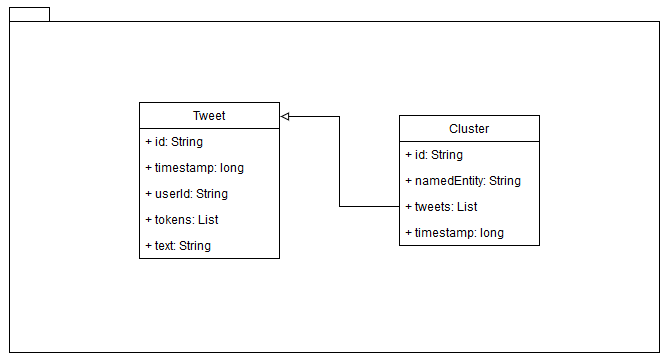
\includegraphics[width=0.5\linewidth]{images/modelUML.png}        
  \caption{UML model classes}
  \label{fig:modelUML}
\end{figure}

Initially, two model classes have been defined, as seen in Figure \ref{fig:modelUML}. The first class, Tweet, contains the appropriate fields for identifying a tweet, such as: tweet ID, timestamp, user ID, parsed tweet tokens and the body text of the tweet. 
Additionally, a second model class defined is Cluster, which references the previous class tweet. Cluster class contains a list of tweets with the same properties and is defined by a cluster ID, by the named entity which are identified by all the tweets and a timestamp which, we'll see in the next paragraphs, will hold the centroid time of all tweets in that specific cluster.\\

The data set is read from local disk through an instance of IOProcessor, which is an interface for reading data.
Since the data set is in CSV format, a class CSVProcessor implementing the IOProcessor interface has been defined. 
It provides methods for reading CSV cluster files and instantiating model classes to be used in the logic of the system.
Diagram for Processor classes can be seen in Figure \ref{fig:processorUML}. \\

\begin{figure}[h!]
    \centering
    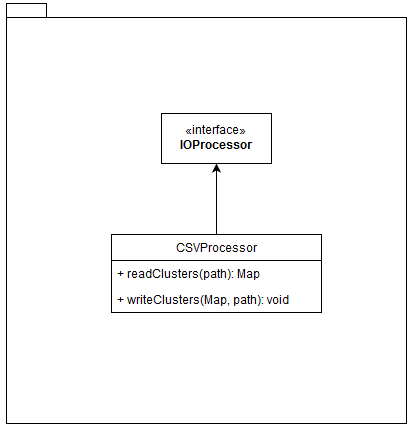
\includegraphics[width=0.5\linewidth]{images/processorUML.png}
  \caption{UML IO processor classes}
  \label{fig:processorUML}
\end{figure}

Data is read and processed as streams of Cluster objects on which multiple sequential operations can be applied. 
ClusterFilter is an interface that can be extended to add more available operations. The available operations, as seen in \ref{fig:filterUML}, are:
\begin{itemize}
    \item NumberOfTweetsFilter - is a class that filters the cluster by a set number of tweets.
    \item CentroidCalculationFilter - provides a method for calculating the centroid time for each cluster within the stream.
    \item MergeNamedEntityFilter - is a filter that merges clusters with the same named entities. A time difference can be set that merges cluster with their centroid time within the same time difference.
\end{itemize}

\begin{figure}[h!]
    \centering
    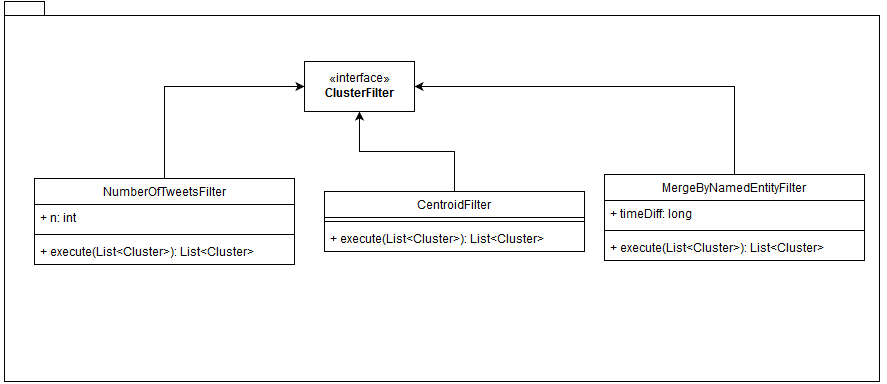
\includegraphics[width=0.7\linewidth]{images/filterUML.png}
  \caption{UML filter classes}
  \label{fig:filterUML}
\end{figure}

Each one of these filters can be applied in any sequence and the entire code can be run into a class containing the main function.
Once all the operations are applied on the stream, the clusters are written back to the file, with the help of CSVProcessor.

\begin{figure}[h!]
    \centering
    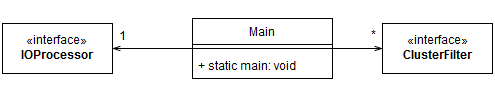
\includegraphics[width=0.7\linewidth]{images/mainUML.png}
  \caption{UML Main class}
  \label{fig:mainUML}
\end{figure}

%%%%%%%%%%%%%%%%%%%%%%%%%%%%%%%%%%%%%%%%%%%%%%%%%%%%%%%%%%%%%%%%%%%%%%%%%%%%%%%%%%
\section{Evaluation}
\begin{enumerate}
    \item Data collection discussion
    \item Explain evaluation measures and report the measures
    \item critically comment on results
\end{enumerate}

%%%%%%%%%%%%%%%%%%%%%%%%%%%%%%%%%%%%%%%%%%%%%%%%%%%%%%%%%%%%%%%%%%%%%%%%%%%%%%%%%%
\section{Discussion}
\begin{enumerate}
    \item scalability, usability, effectiveness, efficiency, etc.
    \item applications of the method
    \item justify with data/information
\end{enumerate}

%%%%%%%%%%%%%%%%%%%%%%%%%%%%%%%%%%%%%%%%%%%%%%%%%%%%%%%%%%%%%%%%%%%%%%%%%%%%%%%%%%
\section{Traffic Event Detection}
\subsection{Problem Statement}
\subsection{Proposed Solution}
\subsection{Discussion}

%==============================================annotated bibliography
\newpage
\nocite{*}
\bibliographystyle{plain}
\bibliography{bibliography}

\end{document}
